\documentclass[10pt,a4paper,noindentfirst]{article}\usepackage[]{graphicx}\usepackage[]{color}
%% maxwidth is the original width if it is less than linewidth
%% otherwise use linewidth (to make sure the graphics do not exceed the margin)
\makeatletter
\def\maxwidth{ %
  \ifdim\Gin@nat@width>\linewidth
    \linewidth
  \else
    \Gin@nat@width
  \fi
}
\makeatother

\definecolor{fgcolor}{rgb}{0.345, 0.345, 0.345}
\newcommand{\hlnum}[1]{\textcolor[rgb]{0.686,0.059,0.569}{#1}}%
\newcommand{\hlstr}[1]{\textcolor[rgb]{0.192,0.494,0.8}{#1}}%
\newcommand{\hlcom}[1]{\textcolor[rgb]{0.678,0.584,0.686}{\textit{#1}}}%
\newcommand{\hlopt}[1]{\textcolor[rgb]{0,0,0}{#1}}%
\newcommand{\hlstd}[1]{\textcolor[rgb]{0.345,0.345,0.345}{#1}}%
\newcommand{\hlkwa}[1]{\textcolor[rgb]{0.161,0.373,0.58}{\textbf{#1}}}%
\newcommand{\hlkwb}[1]{\textcolor[rgb]{0.69,0.353,0.396}{#1}}%
\newcommand{\hlkwc}[1]{\textcolor[rgb]{0.333,0.667,0.333}{#1}}%
\newcommand{\hlkwd}[1]{\textcolor[rgb]{0.737,0.353,0.396}{\textbf{#1}}}%

\usepackage{framed}
\makeatletter
\newenvironment{kframe}{%
 \def\at@end@of@kframe{}%
 \ifinner\ifhmode%
  \def\at@end@of@kframe{\end{minipage}}%
  \begin{minipage}{\columnwidth}%
 \fi\fi%
 \def\FrameCommand##1{\hskip\@totalleftmargin \hskip-\fboxsep
 \colorbox{shadecolor}{##1}\hskip-\fboxsep
     % There is no \\@totalrightmargin, so:
     \hskip-\linewidth \hskip-\@totalleftmargin \hskip\columnwidth}%
 \MakeFramed {\advance\hsize-\width
   \@totalleftmargin\z@ \linewidth\hsize
   \@setminipage}}%
 {\par\unskip\endMakeFramed%
 \at@end@of@kframe}
\makeatother

\definecolor{shadecolor}{rgb}{.97, .97, .97}
\definecolor{messagecolor}{rgb}{0, 0, 0}
\definecolor{warningcolor}{rgb}{1, 0, 1}
\definecolor{errorcolor}{rgb}{1, 0, 0}
\newenvironment{knitrout}{}{} % an empty environment to be redefined in TeX

\usepackage{alltt}

\usepackage[T1]{fontenc}
\usepackage[polish]{babel}
\usepackage[cp1250]{inputenc}
\usepackage{amsmath}
\usepackage{amsfonts}
\usepackage{graphicx}
\usepackage{setspace}
\usepackage{savesym}
\savesymbol{arc}
\usepackage{color}
\usepackage{xcolor}
\usepackage{pict2e}
\usepackage{epstopdf}
\usepackage{geometry}

\newgeometry{tmargin=0.9cm, bmargin=0.9cm, lmargin=0.9cm, rmargin=0.9cm}
\pagestyle{empty}
\linespread{1.2}
\IfFileExists{upquote.sty}{\usepackage{upquote}}{}
\begin{document}

\begin{knitrout}
\definecolor{shadecolor}{rgb}{0.969, 0.969, 0.969}\color{fgcolor}\begin{kframe}
\begin{alltt}
\hlcom{# 1.1}

\hlkwd{library}\hlstd{(}\hlstr{"quantmod"}\hlstd{)}

\hlstd{r} \hlkwb{<-} \hlkwd{read.table}\hlstd{(}\hlstr{"http://gamma.mini.pw.edu.pl/~szymanowskih/lab1/USPOP.DATA"}\hlstd{)}
\hlkwd{head}\hlstd{(r,}\hlnum{3}\hlstd{)}
\end{alltt}
\begin{verbatim}
##        V1
## 1 3929214
## 2 5308483
## 3 7239881
\end{verbatim}
\begin{alltt}
\hlcom{# a)}

\hlstd{USpop} \hlkwb{<-} \hlkwd{ts}\hlstd{(}\hlkwc{data}\hlstd{=r,} \hlkwc{start}\hlstd{=}\hlnum{1790}\hlstd{,} \hlkwc{end}\hlstd{=}\hlnum{1990}\hlstd{,} \hlkwc{frequency}\hlstd{=}\hlnum{0.1}\hlstd{)}

\hlcom{# b)}

\hlkwd{ts.plot}\hlstd{(USpop)}
\end{alltt}
\end{kframe}

{\centering \includegraphics[width=\maxwidth]{figure/unnamed-chunk-11} 

}


\begin{kframe}\begin{alltt}
\hlstd{d} \hlkwb{<-} \hlkwd{diff}\hlstd{(USpop)}
\hlkwd{ts.plot}\hlstd{(d,}\hlkwc{type}\hlstd{=}\hlstr{"b"}\hlstd{)}
\end{alltt}
\end{kframe}

{\centering 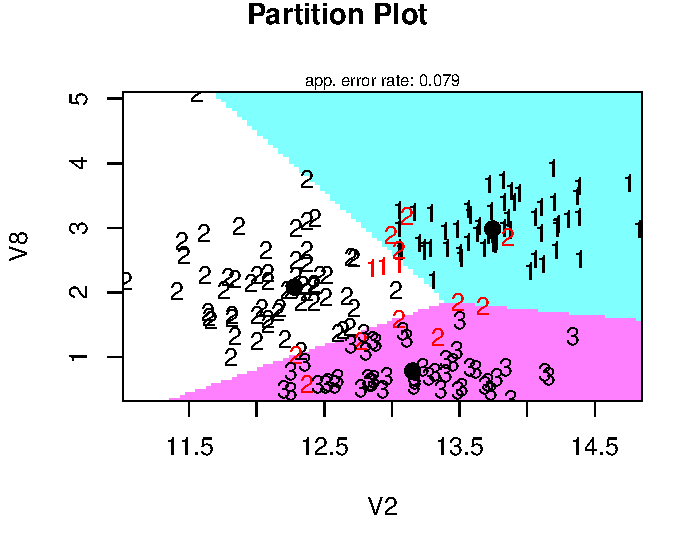
\includegraphics[width=\maxwidth]{figure/unnamed-chunk-12} 

}


\begin{kframe}\begin{alltt}
\hlkwd{which.min}\hlstd{(d)}   \hlcom{# najmniejszy wzrost w latach 1790-1800 }
\end{alltt}
\begin{verbatim}
## [1] 1
\end{verbatim}
\begin{alltt}
\hlcom{# c)}

\hlstd{czas} \hlkwb{<-} \hlkwd{seq}\hlstd{(}\hlkwd{start}\hlstd{(USpop),} \hlkwd{end}\hlstd{(USpop),} \hlkwc{by}\hlstd{=}\hlnum{1}\hlopt{/}\hlkwd{frequency}\hlstd{(USpop))}
\hlstd{m1.lm} \hlkwb{<-} \hlkwd{lm}\hlstd{(USpop} \hlopt{~} \hlstd{czas} \hlopt{+} \hlkwd{I}\hlstd{(czas}\hlopt{^}\hlnum{2}\hlstd{))}
\hlkwd{summary}\hlstd{(m1.lm)}
\end{alltt}
\begin{verbatim}
## 
## Call:
## lm(formula = USpop ~ czas + I(czas^2))
## 
## Residuals:
##      Min       1Q   Median       3Q      Max 
## -6947521  -358167   436285  1481410  3391761 
## 
## Coefficients:
##              Estimate Std. Error t value Pr(>|t|)    
## (Intercept)  2.10e+10   6.59e+08    31.9   <2e-16 ***
## czas        -2.34e+07   6.98e+05   -33.5   <2e-16 ***
## I(czas^2)    6.51e+03   1.85e+02    35.2   <2e-16 ***
## ---
## Signif. codes:  0 '***' 0.001 '**' 0.01 '*' 0.05 '.' 0.1 ' ' 1
## 
## Residual standard error: 2770000 on 18 degrees of freedom
## Multiple R-squared:  0.999,	Adjusted R-squared:  0.999 
## F-statistic: 8.05e+03 on 2 and 18 DF,  p-value: <2e-16
\end{verbatim}
\begin{alltt}
\hlstd{wsp} \hlkwb{<-} \hlkwd{summary}\hlstd{(m1.lm)}\hlopt{$}\hlstd{coefficients[,}\hlnum{1}\hlstd{]}
\end{alltt}
\end{kframe}
\end{knitrout}


\begin{knitrout}
\definecolor{shadecolor}{rgb}{0.969, 0.969, 0.969}\color{fgcolor}\begin{kframe}
\begin{alltt}
\hlkwd{ts.plot}\hlstd{(USpop)}
\hlkwd{curve}\hlstd{(wsp[}\hlnum{1}\hlstd{]}\hlopt{+}\hlstd{wsp[}\hlnum{2}\hlstd{]}\hlopt{*}\hlstd{x}\hlopt{+}\hlstd{wsp[}\hlnum{3}\hlstd{]}\hlopt{*}\hlstd{x}\hlopt{^}\hlnum{2}\hlstd{,}\hlkwc{from}\hlstd{=}\hlnum{1790}\hlstd{,} \hlkwc{to}\hlstd{=}\hlnum{1990}\hlstd{,}\hlkwc{add}\hlstd{=}\hlnum{TRUE}\hlstd{,}\hlkwc{col}\hlstd{=}\hlstr{"red"}\hlstd{)}
\end{alltt}
\end{kframe}

{\centering \includegraphics[width=\maxwidth]{figure/unnamed-chunk-21} 

}


\begin{kframe}\begin{alltt}
\hlcom{# wykres reziduow od czasu:}

\hlkwd{plot}\hlstd{(czas, m1.lm}\hlopt{$}\hlstd{residuals,} \hlkwc{type}\hlstd{=}\hlstr{"b"}\hlstd{)}
\end{alltt}
\end{kframe}

{\centering \includegraphics[width=\maxwidth]{figure/unnamed-chunk-22} 

}



\end{knitrout}


\begin{knitrout}
\definecolor{shadecolor}{rgb}{0.969, 0.969, 0.969}\color{fgcolor}\begin{kframe}
\begin{alltt}
\hlcom{# d)}

\hlstd{res} \hlkwb{<-} \hlstd{m1.lm}\hlopt{$}\hlstd{residuals}
\hlstd{USres} \hlkwb{<-} \hlkwd{ts}\hlstd{(res,} \hlkwc{start}\hlstd{=}\hlnum{1790}\hlstd{,} \hlkwc{end}\hlstd{=}\hlnum{1990}\hlstd{,} \hlkwc{frequency}\hlstd{=}\hlnum{0.1}\hlstd{)}

\hlstd{n} \hlkwb{<-} \hlkwd{length}\hlstd{(USres)}
\hlstd{sr} \hlkwb{<-} \hlkwd{mean}\hlstd{(res)}
\hlstd{autokor} \hlkwb{<-} \hlkwd{numeric}\hlstd{(}\hlnum{14}\hlstd{)}
\hlstd{gamma0} \hlkwb{<-} \hlstd{(}\hlkwd{sum}\hlstd{((res}\hlopt{-}\hlstd{sr)}\hlopt{^}\hlnum{2}\hlstd{))}\hlopt{/}\hlstd{n}
\hlstd{autokor[}\hlnum{1}\hlstd{]} \hlkwb{<-} \hlnum{1}

\hlkwa{for}\hlstd{(i} \hlkwa{in} \hlnum{1}\hlopt{:}\hlnum{13}\hlstd{)\{}
   \hlstd{gammah} \hlkwb{<-} \hlstd{(}\hlkwd{sum}\hlstd{((res[}\hlnum{1}\hlopt{:}\hlstd{(}\hlnum{21}\hlopt{-}\hlstd{i)]}\hlopt{-}\hlstd{sr)}\hlopt{*}\hlstd{(res[(i}\hlopt{+}\hlnum{1}\hlstd{)}\hlopt{:}\hlnum{21}\hlstd{]}\hlopt{-}\hlstd{sr)))}\hlopt{/}\hlstd{n}
   \hlstd{autokor[i}\hlopt{+}\hlnum{1}\hlstd{]} \hlkwb{<-} \hlstd{gammah}\hlopt{/}\hlstd{gamma0}
\hlstd{\}}

\hlkwd{plot}\hlstd{(}\hlnum{1}\hlopt{:}\hlnum{14}\hlstd{,autokor,}\hlkwc{type}\hlstd{=}\hlstr{"h"}\hlstd{)}
\hlstd{kw} \hlkwb{<-} \hlkwd{qnorm}\hlstd{(}\hlnum{0.975}\hlstd{)}\hlopt{/}\hlkwd{sqrt}\hlstd{(n)}
\hlkwd{abline}\hlstd{(}\hlkwc{b}\hlstd{=}\hlnum{0}\hlstd{,}\hlkwc{a}\hlstd{=kw,}\hlkwc{lty}\hlstd{=}\hlnum{2}\hlstd{,}\hlkwc{col}\hlstd{=}\hlstr{"blue"}\hlstd{)}
\hlkwd{abline}\hlstd{(}\hlkwc{b}\hlstd{=}\hlnum{0}\hlstd{,}\hlkwc{a}\hlstd{=}\hlopt{-}\hlstd{kw,}\hlkwc{lty}\hlstd{=}\hlnum{2}\hlstd{,}\hlkwc{col}\hlstd{=}\hlstr{"blue"}\hlstd{)}
\hlkwd{abline}\hlstd{(}\hlkwc{b}\hlstd{=}\hlnum{0}\hlstd{,}\hlkwc{a}\hlstd{=}\hlnum{0}\hlstd{)}
\end{alltt}
\end{kframe}

{\centering \includegraphics[width=\maxwidth]{figure/unnamed-chunk-31} 

}


\begin{kframe}\begin{alltt}
\hlcom{# funkcja wbudowana rysujaca ten sam wykres:}

\hlkwd{acf}\hlstd{(USres)}   \hlcom{# jest autokorelacja rzedu 3 -> testujemy formalnie, czy jest korelacja}
\end{alltt}
\end{kframe}

{\centering \includegraphics[width=\maxwidth]{figure/unnamed-chunk-32} 

}


\begin{kframe}\begin{alltt}
\hlcom{# e)}
\hlcom{# H0: pierwsze 10 korelacji jest rowne zero  }
\hlcom{# lag := h}

\hlkwd{Box.test}\hlstd{(USres,} \hlkwc{lag} \hlstd{=} \hlnum{10}\hlstd{,} \hlkwc{type}\hlstd{=}\hlstr{"Ljung"}\hlstd{)}
\end{alltt}
\begin{verbatim}
## 
## 	Box-Ljung test
## 
## data:  USres
## X-squared = 18.6, df = 10, p-value = 0.04565
\end{verbatim}
\begin{alltt}
\hlcom{# czyli rezidua nie sa bialym szumem niestety}

\hlcom{# 1.2}

\hlkwd{data}\hlstd{(LakeHuron)}
\hlkwd{head}\hlstd{(LakeHuron)}
\end{alltt}
\begin{verbatim}
## [1] 580.4 581.9 581.0 580.8 579.8 580.4
\end{verbatim}
\begin{alltt}
\hlkwd{is.ts}\hlstd{(LakeHuron)}
\end{alltt}
\begin{verbatim}
## [1] TRUE
\end{verbatim}
\end{kframe}
\end{knitrout}

\begin{knitrout}
\definecolor{shadecolor}{rgb}{0.969, 0.969, 0.969}\color{fgcolor}\begin{kframe}
\begin{alltt}
\hlcom{# a)}

\hlkwd{ts.plot}\hlstd{(LakeHuron)}    \hlcom{# widac tendencje malejaca}

\hlcom{# b)}

\hlstd{czas} \hlkwb{<-} \hlkwd{as.vector}\hlstd{(}\hlkwd{time}\hlstd{(LakeHuron))}
\hlstd{lake.lm} \hlkwb{<-} \hlkwd{lm}\hlstd{(LakeHuron} \hlopt{~} \hlstd{czas,} \hlkwc{data}\hlstd{=LakeHuron)}
\hlkwd{abline}\hlstd{(lake.lm,} \hlkwc{col}\hlstd{=}\hlstr{"red"}\hlstd{)}
\end{alltt}
\end{kframe}

{\centering \includegraphics[width=\maxwidth]{figure/unnamed-chunk-41} 

}


\begin{kframe}\begin{alltt}
\hlcom{# c)}

\hlstd{res} \hlkwb{<-} \hlstd{lake.lm}\hlopt{$}\hlstd{residuals}
\hlstd{rszer} \hlkwb{<-} \hlkwd{ts}\hlstd{(}\hlkwc{data}\hlstd{=res)}
\hlkwd{ts.plot}\hlstd{(rszer)}
\end{alltt}
\end{kframe}

{\centering 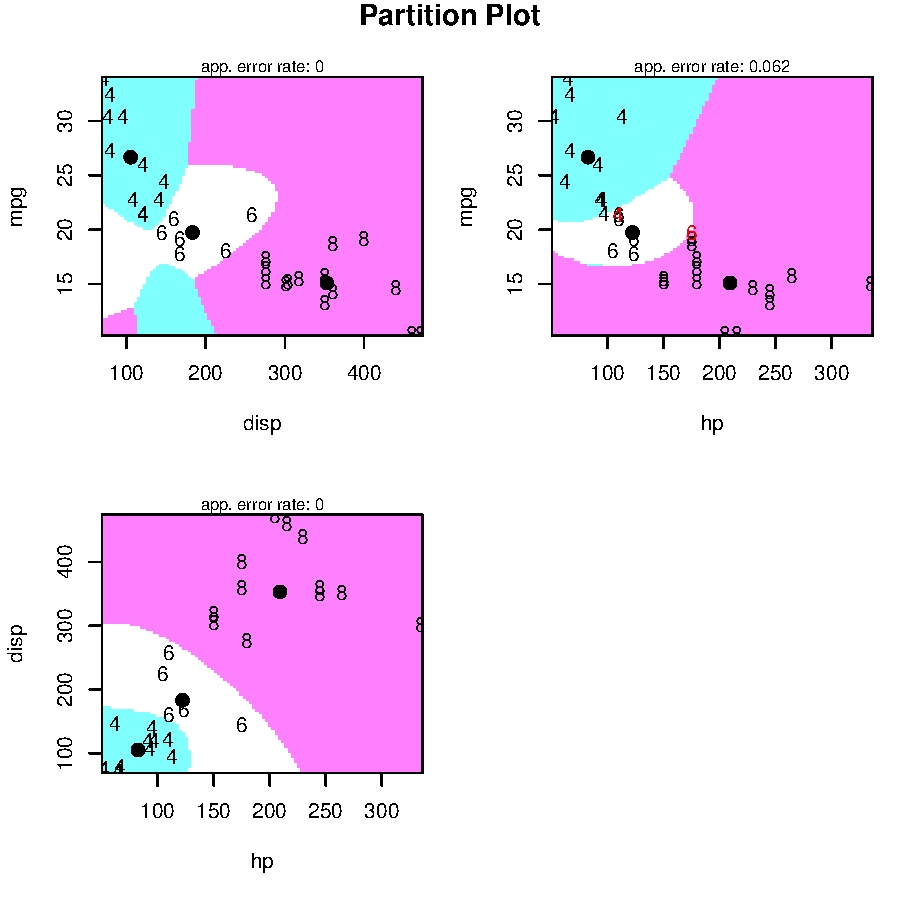
\includegraphics[width=\maxwidth]{figure/unnamed-chunk-42} 

}


\begin{kframe}\begin{alltt}
\hlkwd{acf}\hlstd{(rszer)}   \hlcom{# pasowaloby MA(3)}
\end{alltt}
\end{kframe}

{\centering \includegraphics[width=\maxwidth]{figure/unnamed-chunk-43} 

}


\begin{kframe}\begin{alltt}
\hlkwd{Box.test}\hlstd{(rszer,} \hlkwc{lag} \hlstd{=} \hlnum{20}\hlstd{,} \hlkwc{type}\hlstd{=}\hlstr{"Ljung"}\hlstd{)}
\end{alltt}
\begin{verbatim}
## 
## 	Box-Ljung test
## 
## data:  rszer
## X-squared = 107.8, df = 20, p-value = 4.885e-14
\end{verbatim}
\begin{alltt}
\hlcom{# to zdecydowanie nie jest bialy szum!}

\hlcom{# d)}

\hlstd{r0} \hlkwb{<-} \hlstd{res}
\hlstd{r1} \hlkwb{<-} \hlkwd{Lag}\hlstd{(res,}\hlkwc{k}\hlstd{=}\hlnum{1}\hlstd{)}
\hlstd{r2} \hlkwb{<-} \hlkwd{Lag}\hlstd{(res,}\hlkwc{k}\hlstd{=}\hlnum{2}\hlstd{)}

\hlkwd{head}\hlstd{(r0)}
\end{alltt}
\begin{verbatim}
##       1       2       3       4       5       6 
##  0.2022  1.7064  0.8406  0.6948 -0.2910  0.3332
\end{verbatim}
\begin{alltt}
\hlkwd{head}\hlstd{(r1)}
\end{alltt}
\begin{verbatim}
##        Lag.1
## [1,]      NA
## [2,]  0.2022
## [3,]  1.7064
## [4,]  0.8406
## [5,]  0.6948
## [6,] -0.2910
\end{verbatim}
\begin{alltt}
\hlkwd{head}\hlstd{(r2)}
\end{alltt}
\begin{verbatim}
##       Lag.2
## [1,]     NA
## [2,]     NA
## [3,] 0.2022
## [4,] 1.7064
## [5,] 0.8406
## [6,] 0.6948
\end{verbatim}
\begin{alltt}
\hlcom{# e)}

\hlstd{l} \hlkwb{<-} \hlkwd{lm}\hlstd{(r0}\hlopt{~}\hlstd{r1)}
\hlkwd{summary}\hlstd{(l)}
\end{alltt}
\begin{verbatim}
## 
## Call:
## lm(formula = r0 ~ r1)
## 
## Residuals:
##     Min      1Q  Median      3Q     Max 
## -1.9588 -0.4993  0.0017  0.4178  1.8956 
## 
## Coefficients:
##             Estimate Std. Error t value Pr(>|t|)    
## (Intercept)   0.0153     0.0727    0.21     0.83    
## r1            0.7911     0.0659   12.00   <2e-16 ***
## ---
## Signif. codes:  0 '***' 0.001 '**' 0.01 '*' 0.05 '.' 0.1 ' ' 1
## 
## Residual standard error: 0.716 on 95 degrees of freedom
##   (1 observation deleted due to missingness)
## Multiple R-squared:  0.603,	Adjusted R-squared:  0.599 
## F-statistic:  144 on 1 and 95 DF,  p-value: <2e-16
\end{verbatim}
\begin{alltt}
\hlkwd{mean}\hlstd{(l}\hlopt{$}\hlstd{residuals}\hlopt{^}\hlnum{2}\hlstd{)}    \hlcom{# MSE}
\end{alltt}
\begin{verbatim}
## [1] 0.5022
\end{verbatim}
\begin{alltt}
\hlkwd{acf}\hlstd{(l}\hlopt{$}\hlstd{res)}
\end{alltt}
\end{kframe}

{\centering \includegraphics[width=\maxwidth]{figure/unnamed-chunk-44} 

}


\begin{kframe}\begin{alltt}
\hlkwd{Box.test}\hlstd{(l}\hlopt{$}\hlstd{res,}\hlkwc{lag}\hlstd{=}\hlnum{20}\hlstd{,}\hlkwc{type}\hlstd{=}\hlstr{"Ljung"}\hlstd{)}
\end{alltt}
\begin{verbatim}
## 
## 	Box-Ljung test
## 
## data:  l$res
## X-squared = 19.71, df = 20, p-value = 0.4765
\end{verbatim}
\begin{alltt}
\hlcom{# f)}

\hlstd{l2} \hlkwb{<-} \hlkwd{lm}\hlstd{(r0}\hlopt{~}\hlstd{r1}\hlopt{+}\hlstd{r2)}
\hlkwd{summary}\hlstd{(l2)}
\end{alltt}
\begin{verbatim}
## 
## Call:
## lm(formula = r0 ~ r1 + r2)
## 
## Residuals:
##     Min      1Q  Median      3Q     Max 
## -1.5843 -0.4525 -0.0162  0.4030  1.7320 
## 
## Coefficients:
##             Estimate Std. Error t value Pr(>|t|)    
## (Intercept) -0.00785    0.06912   -0.11   0.9098    
## r1           1.00214    0.09722   10.31   <2e-16 ***
## r2          -0.28380    0.09900   -2.87   0.0051 ** 
## ---
## Signif. codes:  0 '***' 0.001 '**' 0.01 '*' 0.05 '.' 0.1 ' ' 1
## 
## Residual standard error: 0.677 on 93 degrees of freedom
##   (2 observations deleted due to missingness)
## Multiple R-squared:  0.644,	Adjusted R-squared:  0.636 
## F-statistic: 84.2 on 2 and 93 DF,  p-value: <2e-16
\end{verbatim}
\begin{alltt}
\hlkwd{mean}\hlstd{(l2}\hlopt{$}\hlstd{residuals}\hlopt{^}\hlnum{2}\hlstd{)}
\end{alltt}
\begin{verbatim}
## [1] 0.4435
\end{verbatim}
\begin{alltt}
\hlkwd{acf}\hlstd{(l2}\hlopt{$}\hlstd{res)}
\end{alltt}
\end{kframe}

{\centering \includegraphics[width=\maxwidth]{figure/unnamed-chunk-45} 

}


\begin{kframe}\begin{alltt}
\hlkwd{Box.test}\hlstd{(l2}\hlopt{$}\hlstd{res,}\hlkwc{lag}\hlstd{=}\hlnum{20}\hlstd{,}\hlkwc{type}\hlstd{=}\hlstr{"Ljung"}\hlstd{)}  \hlcom{# lepiej dopasowany niz l}
\end{alltt}
\begin{verbatim}
## 
## 	Box-Ljung test
## 
## data:  l2$res
## X-squared = 9.033, df = 20, p-value = 0.9825
\end{verbatim}
\begin{alltt}
\hlcom{# g)}

\hlstd{model_ar1} \hlkwb{<-} \hlkwd{arima}\hlstd{(r0,}\hlkwd{c}\hlstd{(}\hlnum{1}\hlstd{,}\hlnum{0}\hlstd{,}\hlnum{0}\hlstd{))}
\hlstd{model_ar2} \hlkwb{<-} \hlkwd{arima}\hlstd{(r0,}\hlkwd{c}\hlstd{(}\hlnum{2}\hlstd{,}\hlnum{0}\hlstd{,}\hlnum{0}\hlstd{))}

\hlkwd{Box.test}\hlstd{(model_ar1}\hlopt{$}\hlstd{residuals,}\hlkwc{lag}\hlstd{=}\hlnum{20}\hlstd{,}\hlkwc{type}\hlstd{=}\hlstr{"Ljung"}\hlstd{)}
\end{alltt}
\begin{verbatim}
## 
## 	Box-Ljung test
## 
## data:  model_ar1$residuals
## X-squared = 19.92, df = 20, p-value = 0.4631
\end{verbatim}
\begin{alltt}
\hlkwd{Box.test}\hlstd{(model_ar2}\hlopt{$}\hlstd{residuals,}\hlkwc{lag}\hlstd{=}\hlnum{20}\hlstd{,}\hlkwc{type}\hlstd{=}\hlstr{"Ljung"}\hlstd{)}
\end{alltt}
\begin{verbatim}
## 
## 	Box-Ljung test
## 
## data:  model_ar2$residuals
## X-squared = 8.466, df = 20, p-value = 0.9883
\end{verbatim}
\begin{alltt}
\hlcom{# h)}

\hlstd{model_ar1}
\end{alltt}
\begin{verbatim}
## 
## Call:
## arima(x = r0, order = c(1, 0, 0))
## 
## Coefficients:
##         ar1  intercept
##       0.783      0.080
## s.e.  0.063      0.318
## 
## sigma^2 estimated as 0.497:  log likelihood = -105.3,  aic = 216.6
\end{verbatim}
\begin{alltt}
\hlstd{l}\hlopt{$}\hlstd{coefficients}    \hlcom{# ok, w miare podobne}
\end{alltt}
\begin{verbatim}
## (Intercept)          r1 
##     0.01529     0.79112
\end{verbatim}
\begin{alltt}
\hlcom{# 1.3}

\hlstd{d} \hlkwb{<-} \hlkwd{read.table}\hlstd{(}\hlstr{"C:\textbackslash{}\textbackslash{}Users\textbackslash{}\textbackslash{}Marta\textbackslash{}\textbackslash{}Desktop\textbackslash{}\textbackslash{}Marta\textbackslash{}\textbackslash{}studia\textbackslash{}\textbackslash{}rok4\textbackslash{}\textbackslash{}Szeregi czasowe\textbackslash{}\textbackslash{}DOWJ.DAT"}\hlstd{)}
\hlkwd{head}\hlstd{(d)}
\end{alltt}
\begin{verbatim}
##      V1
## 1 110.9
## 2 110.7
## 3 110.4
## 4 110.6
## 5 110.8
## 6 110.8
\end{verbatim}
\begin{alltt}
\hlcom{# a)}

\hlstd{t} \hlkwb{<-} \hlkwd{ts}\hlstd{(}\hlkwc{data}\hlstd{=d)}

\hlcom{# b)}

\hlkwd{plot}\hlstd{(t)}    \hlcom{# widoczny jest trend!!!}
\end{alltt}
\end{kframe}

{\centering \includegraphics[width=\maxwidth]{figure/unnamed-chunk-46} 

}


\begin{kframe}\begin{alltt}
\hlcom{# c)}

\hlkwd{acf}\hlstd{(t)}     \hlcom{# szereg niestacjonarny -> zeby sie pozbyc trendu roznicujemy}
\end{alltt}
\end{kframe}

{\centering \includegraphics[width=\maxwidth]{figure/unnamed-chunk-47} 

}


\begin{kframe}\begin{alltt}
\hlcom{# d)}

\hlstd{dd} \hlkwb{<-} \hlkwd{diff}\hlstd{(}\hlkwd{as.numeric}\hlstd{(}\hlkwd{as.matrix}\hlstd{(d)))}
\hlstd{tt} \hlkwb{<-} \hlkwd{ts}\hlstd{(}\hlkwc{data}\hlstd{=dd)}

\hlcom{# e)}

\hlkwd{ts.plot}\hlstd{(tt)}
\end{alltt}
\end{kframe}

{\centering \includegraphics[width=\maxwidth]{figure/unnamed-chunk-48} 

}


\begin{kframe}\begin{alltt}
\hlkwd{Box.test}\hlstd{(tt,}\hlkwc{lag}\hlstd{=}\hlnum{20}\hlstd{,}\hlkwc{type}\hlstd{=}\hlstr{"Ljung"}\hlstd{)}
\end{alltt}
\begin{verbatim}
## 
## 	Box-Ljung test
## 
## data:  tt
## X-squared = 46.43, df = 20, p-value = 0.0007039
\end{verbatim}
\begin{alltt}
\hlcom{# f)}

\hlkwd{acf}\hlstd{(tt)}   \hlcom{# sugeruje model MA(2)}
\end{alltt}
\end{kframe}

{\centering \includegraphics[width=\maxwidth]{figure/unnamed-chunk-49} 

}


\begin{kframe}\begin{alltt}
\hlkwd{pacf}\hlstd{(tt)}  \hlcom{# sugeruje model AR(1)}
\end{alltt}
\end{kframe}

{\centering \includegraphics[width=\maxwidth]{figure/unnamed-chunk-410} 

}


\begin{kframe}\begin{alltt}
\hlstd{ma2} \hlkwb{<-} \hlkwd{arima}\hlstd{(dd,}\hlkwd{c}\hlstd{(}\hlnum{0}\hlstd{,}\hlnum{0}\hlstd{,}\hlnum{2}\hlstd{))}
\hlstd{ar1} \hlkwb{<-} \hlkwd{arima}\hlstd{(dd,}\hlkwd{c}\hlstd{(}\hlnum{1}\hlstd{,}\hlnum{0}\hlstd{,}\hlnum{0}\hlstd{))}
\hlstd{arma12} \hlkwb{<-} \hlkwd{arima}\hlstd{(dd,}\hlkwd{c}\hlstd{(}\hlnum{1}\hlstd{,}\hlnum{0}\hlstd{,}\hlnum{2}\hlstd{))}

\hlkwd{Box.test}\hlstd{(ma2}\hlopt{$}\hlstd{res,}\hlkwc{lag}\hlstd{=}\hlnum{20}\hlstd{,}\hlkwc{type}\hlstd{=}\hlstr{"Ljung"}\hlstd{)}
\end{alltt}
\begin{verbatim}
## 
## 	Box-Ljung test
## 
## data:  ma2$res
## X-squared = 31.4, df = 20, p-value = 0.05011
\end{verbatim}
\begin{alltt}
\hlkwd{Box.test}\hlstd{(ar1}\hlopt{$}\hlstd{res,}\hlkwc{lag}\hlstd{=}\hlnum{20}\hlstd{,}\hlkwc{type}\hlstd{=}\hlstr{"Ljung"}\hlstd{)}
\end{alltt}
\begin{verbatim}
## 
## 	Box-Ljung test
## 
## data:  ar1$res
## X-squared = 32.55, df = 20, p-value = 0.03774
\end{verbatim}
\begin{alltt}
\hlkwd{Box.test}\hlstd{(arma12}\hlopt{$}\hlstd{res,}\hlkwc{lag}\hlstd{=}\hlnum{20}\hlstd{,}\hlkwc{type}\hlstd{=}\hlstr{"Ljung"}\hlstd{)}
\end{alltt}
\begin{verbatim}
## 
## 	Box-Ljung test
## 
## data:  arma12$res
## X-squared = 27.95, df = 20, p-value = 0.1105
\end{verbatim}
\begin{alltt}
\hlkwd{acf}\hlstd{(arma12}\hlopt{$}\hlstd{residuals)}
\end{alltt}
\end{kframe}

{\centering \includegraphics[width=\maxwidth]{figure/unnamed-chunk-411} 

}



\end{knitrout}


\end{document}
